\section{Traffic Volume}

In this section, users can access and filter traffic data based on different traffic types. The available traffic types include various communication channels, allowing users to gain insights into their network's usage and performance. The data can be filtered by the following traffic types:

\begin{itemize}
  \item \textbf{Voice:} Traffic related to voice communications across the network.
  \item \textbf{SMS:} Traffic for short message service (SMS) exchanges, typically for mobile messaging.
  \item \textbf{Data:} Data traffic associated with internet and data transmission over the network.
  \item \textbf{ICX In/Out:} Traffic for International Exchange (ICX), covering both inbound and outbound connections.
  \item \textbf{IGW In/Out:} Traffic related to Internet Gateway (IGW), covering both inbound and outbound data.
\end{itemize}

\vspace{3mm}
\subsection{Traffic Volume-Search}
The common search area will include options to filter by these traffic types, and specific subsections will be added for each traffic category (Voice, SMS, Data, ICX In/Out, IGW In/Out).
In this section, the user can filter traffic volume data by selecting the appropriate parameters from the following options: \\
\:

\textbf{Traffic Type:} The user can select from the following options:

\begin{figure}[ht]

  \begin{minipage}[b]{0.20\textwidth}
    \begin{itemize}
      \item Voice
      \item SMS
      \item Data
      \item ICX In/Out
      \item IGW In/Out
    \end{itemize}
  \end{minipage}
  \hfill
  \begin{minipage}[t]{0.35\textwidth}
    \centering
    \colorbox{gray!20}{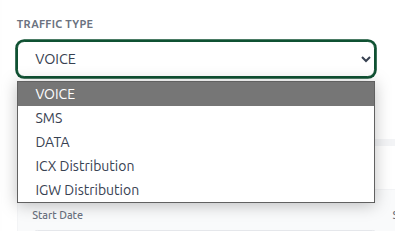
\includegraphics[width=0.95\textwidth]{img/traffic/trafficTypes.png}}
    \caption{Traffic Type Selection}
  \end{minipage}

\end{figure}
\vspace{3mm} %3mm vertical space
\textbf{Period:} The user can select a time period for data view, which can be one of the following:
\vspace{-10pt}
\begin{figure}[h]
  \begin{minipage}[b]{0.40\textwidth}

    \begin{itemize}
      \item Hourly
      \item Daily
      \item Monthly
      \item Yearly
    \end{itemize}
  \end{minipage}
  \hfill
  \begin{minipage}[t]{0.35\textwidth}
    \centering
    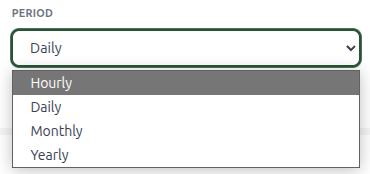
\includegraphics[width=\textwidth]{img/common/commonarea/period.png}  % Replace with the path to your image file
    \caption{Example of Period Selection}
  \end{minipage}
\end{figure}\\
\vfill
\clearpage
\vspace{3mm} %3mm vertical space
\textbf{Quick Presets:} The user can quickly select a preset time range from the following options:

\begin{figure}[h]

  \begin{minipage}[]{0.40\textwidth}
    \begin{itemize}
      \item Last Hour
      \item Last 24 Hours
      \item Last 7 Days
      \item Last 30 Days
      \item Last 90 Days
      \item Last Year
    \end{itemize}
  \end{minipage}
  \begin{minipage}[t]{0.45\textwidth}
    \centering
    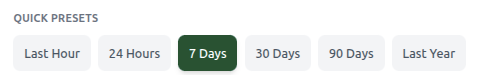
\includegraphics[width=\textwidth]{img/common/commonarea/QuickPresents.png}  % Replace with the path to your image file
    \caption{Example of Quick Preset Selection}
  \end{minipage}

\end{figure}
\vfill

\vspace{3mm} %3mm vertical space
\textbf{Start \& End Date and Time:} The user selects the start date and, if the "Hourly" period is selected, the start time. The end date and end time are also configurable, but the start and end time are only active for the "Hourly" period.\\
\begin{figure}[htbp]
  \centering
  \begin{subfigure}[b]{0.40\textwidth}
    \centering
    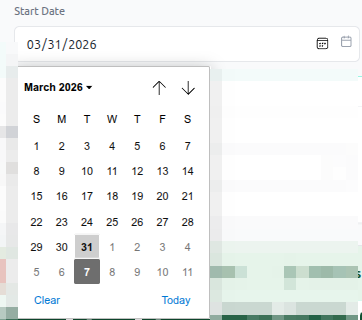
\includegraphics[width=\linewidth,valign=b]{img/common/commonarea/StartDate.png}
    \caption{Start \& End Date Selection}
    \label{fig:img1}
  \end{subfigure}
  \hfill
  \begin{subfigure}[b]{0.40\textwidth}
    \centering
    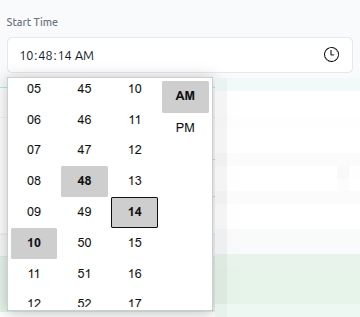
\includegraphics[width=\linewidth,valign=b]{img/common/commonarea/StartTime.png}
    \caption{Start \& End Time Selection}
    \label{fig:img2}
  \end{subfigure}
  \caption{Overall figure caption (optional).}
  \label{fig:side_by_side}
\end{figure}
\vfill
\textbf{Quick Time Selection}

In this section, users can quickly set the desired time range for their data analysis. By using the time selection slider, users can adjust the range by simply moving the indicator along the timeline. This allows for a smooth and intuitive way to select specific periods for viewing data. The slider lets users choose from various predefined time frames, such as Last Hour, Last 24 Hours, and more.

\begin{figure}[h]
  \centering
  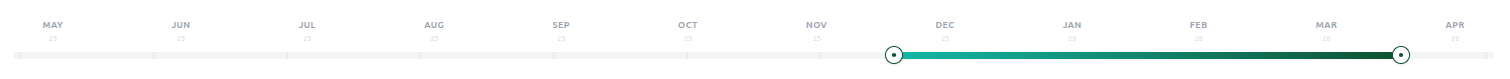
\includegraphics[width=\textwidth]{img/common/commonarea/QuickTimeSelection.png}
  \caption{Example of Quick Time Selection}
\end{figure}

As the user moves the slider, the time range is automatically updated, reflecting the selected period. This feature provides a dynamic and user-friendly interface for analyzing data across different time intervals.
\clearpage

\vspace{5mm} %3mm vertical space
\textbf{Operators:} The user can select operators as needed. The options include:
\begin{itemize}
  \item All operators
  \item Single operator
  \item Multiple operators
\end{itemize}

\vspace{3mm}
\textbf{Network Category:} The user can choose from various network categories, with all categories being selected by default.\linebreak
\begin{figure}[ht]
  \centering
  \itshape
  \colorbox{gray!20}{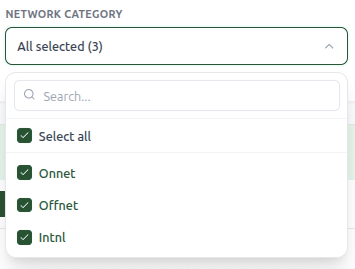
\includegraphics[width=0.35\textwidth]{img/traffic/NetworkCatagory.png}}
  \caption{Example of Network Category Selection}
\end{figure}
\clearpage

\vspace{3mm}
\textbf{Direction:} The user can choose the direction for the traffic (Incoming or Outgoing), with all directions being selected by default.\\
\begin{figure}[ht]
  \centering
  \itshape
  \colorbox{gray!20}{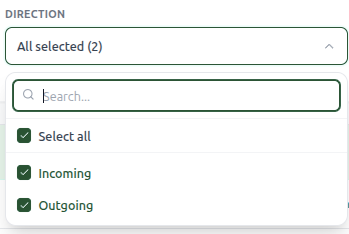
\includegraphics[width=0.30\textwidth]{img/traffic/trafficDirection.png}}
  \caption{Example of Traffic Direction Selection}
\end{figure}
\vspace{3mm}
\textbf{Units:} The user can select between two unit types:
\begin{itemize}
  \item Minute
  \item Count
\end{itemize}

After \textbf{APPLY FILTERS},
\includegraphics[width=0.3\textwidth]{img/common/commonarea/Applyfilter.png} the search results will update to reflect the selected parameters.
